\documentclass[12pt]{article}

\usepackage{bm,amsthm,amssymb,amsfonts,mathtools}
\usepackage[margin=1in]{geometry} 
\usepackage{dsfont}
% neural net drawing
\usepackage{tikz}
\usetikzlibrary{positioning}

\usepackage{neuralnetwork}

% macros
\newcommand{\norm}[1]{\left\lVert#1\right\rVert}

\usepackage{amsmath,amssymb,amsthm,amsfonts,amscd}
\usepackage{showlabels}
\usepackage{color}
\usepackage{hyperref}
\usepackage[numeric]{amsrefs}
\usepackage{graphicx}

\usepackage[framemethod=TikZ]{mdframed}
%\usepackage[framemethod=default]{mdframed}


%\mdfdefinestyle{box}{%
%rightline=true,
%innerleftmargin=10,
%innerrightmargin=10,
%frametitlerule=true,
%frametitlerulecolor=blue,
%frametitlebackgroundcolor=white,
%frametitlerulewidth=2pt}

\mdfdefinestyle{TheoremFrame}{%
    linecolor=blue,
    outerlinewidth=1,
    roundcorner=15,
    innertopmargin= \baselineskip,
    innerbottommargin= \baselineskip,
    innerrightmargin=10,
    innerleftmargin=10,
    backgroundcolor=white}
    
\mdfdefinestyle{ProofFrame}{%
    linecolor=red,
    outerlinewidth=1,
    roundcorner=15,
    innertopmargin= \baselineskip,
    innerbottommargin= \baselineskip,
    innerrightmargin=10,
    innerleftmargin=10,
    backgroundcolor=white}
    
    
\setlength{\oddsidemargin}{0cm}
\setlength{\evensidemargin}{0cm}
\setlength{\marginparwidth}{0in}
\setlength{\marginparsep}{0in}
\setlength{\marginparpush}{0in}
\setlength{\topmargin}{0in}
\setlength{\headheight}{0pt}
\setlength{\headsep}{0pt}
\setlength{\footskip}{.3in}
\setlength{\textheight}{9.2in}
\setlength{\textwidth}{6.0in}
\setlength{\parskip}{0.25pt}
\setlength{\parindent}{0.25in}

    
\newlength\tindent
\setlength{\tindent}{\parindent}
\setlength{\parindent}{0pt}
\renewcommand{\indent}{\hspace*{\tindent}}

\newtheorem*{nthm}{Theorem}
\newtheorem*{nlem}{Lemma}
\newtheorem*{nprop}{Proposition}
\newtheorem*{ncor}{Corollary}
\newtheorem*{nconj}{Conjecture}
\newtheorem*{nclaim}{Claim}
\theoremstyle{remark}
\newtheorem*{define}{Definition}
\newtheorem*{nrem}{Remarks}
\newtheorem*{notation}{Notation}
\newtheorem*{note}{Note}
\newtheorem*{ex}{Example}
\newtheorem*{imt}{Important}
\newtheorem*{fact}{Fact}
\newcommand{\vs}{\vspace{0.1in}}
\newcommand{\Lim}[1]{\raisebox{0.5ex}{\scalebox{0.8}{$\displaystyle \lim_{#1}\;$}}}
\title{Related Rates}
\author{Stephen Styles}
\begin{document}
\maketitle


\begin{enumerate}
\item A dump-truck is pouring sand onto a pile at a rate of $0.5m^3/\text{min}$. The pile of sand is the shape of a cone whose base is always the same length as the height. How fast is the pile increasing when the height is $4\text{cm}$.
\begin{mdframed}[style=TheoremFrame]
\textit{Solution}:\\

The volume for a cone at time $t$ is given by 
\begin{align*}
V(t) = \frac{1}{3} \pi r(t)^2 h(t).
\end{align*}
Since we know that the diameter is always the same as the height, we can replace $r(t)$ with $\frac{1}{2}h(t)$.
\begin{align*}
2r(t) &= h(t)\\
\Rightarrow r(t) &= \frac{1}{2} h(t)
\end{align*}
We can plug this back into the original volume equation to get
\begin{align*}
V(t) &= \frac{1}{3} \pi r(t)^2 h(t)\\
&= \frac{1}{3} \pi \bigg(\frac{1}{2} h(t)\bigg)^2 h(t)\\
&= \frac{\pi}{12}h(t)^3.
\end{align*}
Differentiating both sides we get
\begin{align*}
\frac{dV(t)}{dt} = \frac{3\pi}{12}h(t)^2 \frac{dh(t)}{dt}.
\end{align*}
Plugging our known values into this equation we can solve for the rate of change of the height.
\begin{align*}
0.5 &= \frac{\pi}{4} \cdot 4^2 \cdot \frac{dh(t)}{dt}\\
\Rightarrow \frac{dh(t)}{dt} &= 0.5 \cdot \frac{1}{4\pi}\\
&= \frac{1}{8\pi}
\end{align*}
\end{mdframed}
\item A baseball player is currently on first base. He starts running from first base to second base at a rate of $30\text{feet}/\text{sec}$. How fast is the distance between him and homeplate changing when the player is $45$ feet off first base?
\begin{mdframed}[style=TheoremFrame]
\textit{Solution}:\\

Looking at a picture of a baseball diamond,
\begin{center}
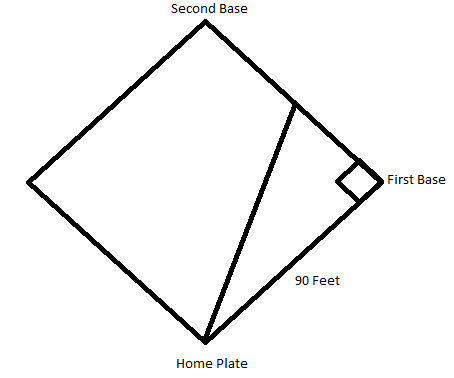
\includegraphics[scale=0.35]{BaseballDiamond}
\end{center}
we can see that the distance between the plater and homeplate is given by the Pythagorean Theorem.\\

Let us denote $x(t) =$ the distance between the player and first base.\\
$z(t) =$ the distance between the player and homeplate.\\

\begin{align*}
x(t)^2 + 90^2 &= z(t)^2
\end{align*}
Taking the derivative of both sides yields
\begin{align*}
2x(t) \frac{dx(t)}{dt} &= 2z(t)\frac{dz(t)}{dt}\\
\Rightarrow \frac{dz(t)}{dt} &= \frac{x(t)}{z(t)} \frac{dx(t)}{dt}
\end{align*}
We can solve for $z(t)$ from the Pythagorean theorem
\begin{align*}
90^2 + 45^2 &= z(t)^2\\
\Rightarrow z(t) &= \sqrt{90^2+45^2}.
\end{align*}
Now we have all the information needed to solve the question. So the rate of change of the distance between the plater and homeplate is 
\begin{align*}
\frac{dz(t)}{dt} &= \frac{x(t)}{z(t)} \frac{dx(t)}{dt}\\
&= \frac{45}{\sqrt{90^2+45^2}} \cdot 30\\
&= 13.42
\end{align*}
\end{mdframed}
\item A spherical snowball melts at a rate of $2\pi \text{cm}^3/\text{hr}$. It melts symmetrically such that it is always a sphere. How fast is its radius changing at the instant\\ $r=10$.
\begin{mdframed}[style=TheoremFrame]
\textit{Solution}:\\

The volume of a sphere is given by
\begin{align*}
V(t) &= \frac{4}{3} \pi r(t)^3.
\end{align*}
Taking the derivative on both sides gets us
\begin{align*}
\frac{dV(t)}{dt} &= 4\pi r(t)^2 \frac{dr(t)}{dt}.
\end{align*}
Which now we can plug in all the values we are given in the question to solve for the rate of change of the radius.
\begin{align*}
2\pi &= 4\pi \cdot 10^2 \cdot \frac{dr(t)}{dt}\\
\Rightarrow \frac{dr(t)}{dt} &= \frac{1}{200}.
\end{align*}
\end{mdframed}
\item A tank of water the shape of a cone is being drained with water at a rate of $15m^3/\text{min}$. The base radius is $27$ meters and the height is $9$ meters. At what rate is the depth of water changing when the radius of the top of the water is $12$ meters.
\begin{mdframed}[style=TheoremFrame]
\textit{Solution}:\\

From question $1$, we know that the volume of a cone is given by
\begin{align*}
V(t) &= \frac{1}{3} \pi r(t)^2 h(t).
\end{align*}
Since this is a product of two functions $h(t)$ and $r(t)$, we will need to rewrite one of the functions in terms of the other. Since we care about the rate of change of the height, we will try to rewrite the radius as a function of the height. Using our similar triangles, we know that
\begin{center}
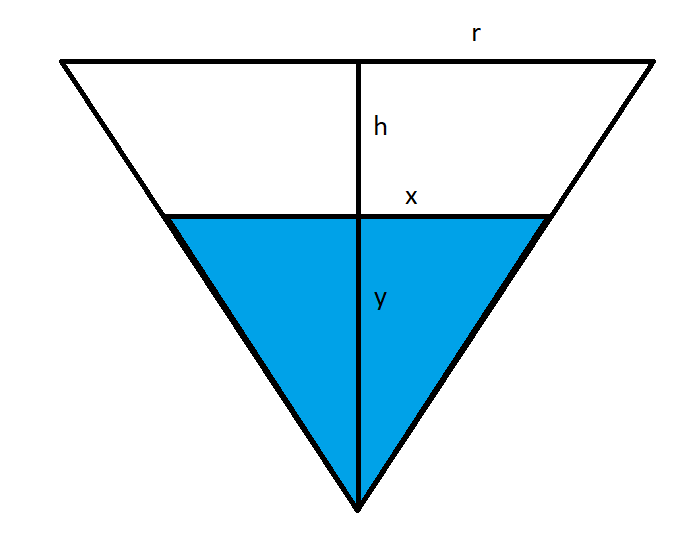
\includegraphics[scale=0.5]{simtriangles}
\end{center}
\begin{align*}
\frac{x}{y} &= \frac{h}{r} = \frac{9}{27} = \frac{1}{3}\\
\Rightarrow \frac{h(t)}{r(t)} &= \frac{1}{3}\\
\Rightarrow r(t) &= 3h(t)
\end{align*}
Substituting this back into our volume formula we get
\begin{align*}
V(t) &= \frac{1}{3} \pi (3 h(t))^2 h(t)\\
&= 3\pi h(t)^3\\
\end{align*}
Taking the derivative of both sides gives us
\begin{align*}
\frac{dV(t)}{dt} &= 3\pi \cdot 3h(t)^2 \frac{dh(t)}{dt}\\
&= 9\pi h(t)^2 \frac{dh(t)}{dt}.
\end{align*}
We can also solve for what the height would be using our similar triangles:
\begin{align*}
\frac{h(t)}{12} &= \frac{1}{3}\\
\Rightarrow h(t) &= 4. 
\end{align*}
Now we can solve for the rate of change of the height
\begin{align*}
\frac{dV(t)}{dt}&= 9\pi h(t)^2 \frac{dh(t)}{dt}\\
\Rightarrow \frac{dh(t)}{dt} &= \frac{dV(t)}{dt} \frac{1}{9\pi h(t)^2}\\
&= -15 \bigg(\frac{1}{9\cdot4^2}\bigg)\\
&= \frac{-15}{144}
\end{align*}
\end{mdframed}
\item The angle of elevation is the angle formed by a horizontal line and a line joining the observers eye to an object above the horizontal line. A person is $5$km away from a launch pad for a rocket. The rocket is blasting off at a rate of $8$km/s. At what rate is the angle of elevation $\theta$, changing when the rocket is $40$km above the ground.
\begin{mdframed}[style=TheoremFrame]
\textit{Solution}:\\

\begin{center}
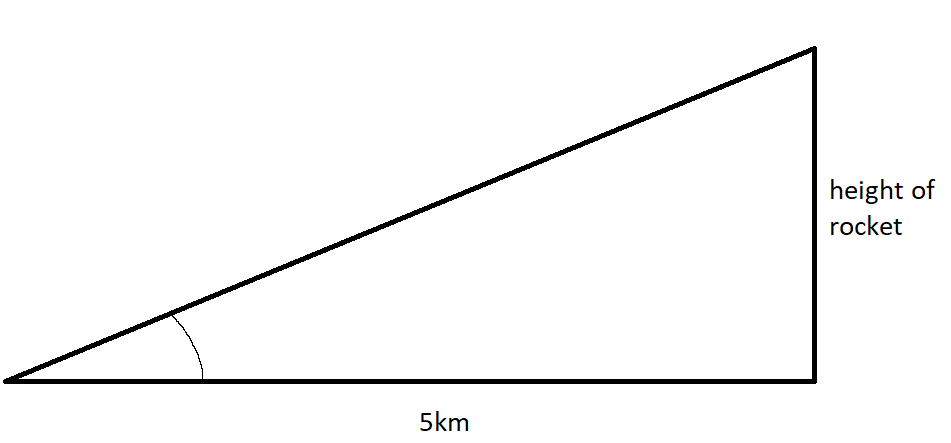
\includegraphics[scale=0.5]{Rocketangle}
\end{center}
The angle of elevation, $\theta(t)$, is given by
\begin{align*}
\tan\big(\theta(t)\big) &= \frac{h(t)}{5}.
\end{align*} 
Taking the derivative of both sides
\begin{align*}
\sec^2\big(\theta(t)\big) \frac{d\theta(t)}{dt}&= \frac{1}{5} \frac{dh(t)}{dt}\\
\Rightarrow \frac{d\theta(t)}{dt} &= \frac{1}{5\sec^2\big(\theta(t)\big)} \frac{dh(t)}{dt}
\end{align*}
We can solve for $\theta(t)$ from the information given in the question
\begin{align*}
\tan\big(\theta(t)\big) &= \frac{40}{5} = 8\\
\Rightarrow \theta(t) &= \tan^{-1}(8)
&\approx 1.45
\end{align*}
Therefore the rate of change of the angle becomes
\begin{align*}
\frac{d\theta(t)}{dt} &= \frac{1}{5\sec^2\big(\theta(t)\big)} \frac{dh(t)}{dt}\\
&= \frac{1}{5 \sec^2(1.45)} \cdot 8\\
&= 0.023
\end{align*}
\end{mdframed}
\end{enumerate}
\end{document}